\documentclass[aspectratio=169]{beamer}
\usetheme{Madrid}
\usecolortheme{default}

% Remove navigation symbols and header/footer
\setbeamertemplate{navigation symbols}{}
\setbeamertemplate{headline}{}
\setbeamertemplate{footline}{
  \hbox{%
  \begin{beamercolorbox}[wd=.5\paperwidth,ht=2.25ex,dp=1ex,left]{author in head/foot}%
    \usebeamerfont{author in head/foot}\hspace*{2ex}\insertshortauthor
  \end{beamercolorbox}%
  \begin{beamercolorbox}[wd=.5\paperwidth,ht=2.25ex,dp=1ex,right]{date in head/foot}%
    \usebeamerfont{date in head/foot}\insertframenumber{} / \inserttotalframenumber\hspace*{2ex}
  \end{beamercolorbox}}%
  \vskip0pt%
}

% Packages
\usepackage{graphicx}
\usepackage{booktabs}
\usepackage{amsmath}
\usepackage{hyperref}
\usepackage{xcolor}

% Custom colors for highlighting
\definecolor{winnergreen}{RGB}{34, 139, 34}
\definecolor{alertred}{RGB}{178, 34, 34}

% Title Information
\title[Stablecoin Stability Analysis]{Stablecoin Stability Analysis}
\subtitle{Predicting Depeg Risk with Machine Learning}
\author{Eymen Celikturk \and Halil Utku Celik}
\institute{CMPE 481 -- Introduction to Data Analysis and Visualization\\Boğaziçi University}
\date{December 2024}

\begin{document}

% Slide 1: Title Slide
\begin{frame}
\titlepage
\end{frame}

% Slide 2: Motivation
\begin{frame}{Why Stablecoin Stability Matters}
\begin{columns}[t]
\column{0.55\textwidth}
\textbf{The Problem:}
\begin{itemize}
    \item Stablecoins are designed to maintain a \$1.00 peg
    \item \textbf{Depeg events} cause massive financial losses
    \item UST/LUNA crash (May 2022): \$40B+ wiped out
    \item USDC depeg (March 2023): dropped to \$0.87
\end{itemize}

\vspace{0.3cm}
\textbf{Our Goal:}
\begin{itemize}
    \item Detect anomalous price behavior early
    \item Predict stability risk 1 hour ahead
    \item Understand market regime patterns
\end{itemize}

\column{0.45\textwidth}
\begin{figure}
    \centering
    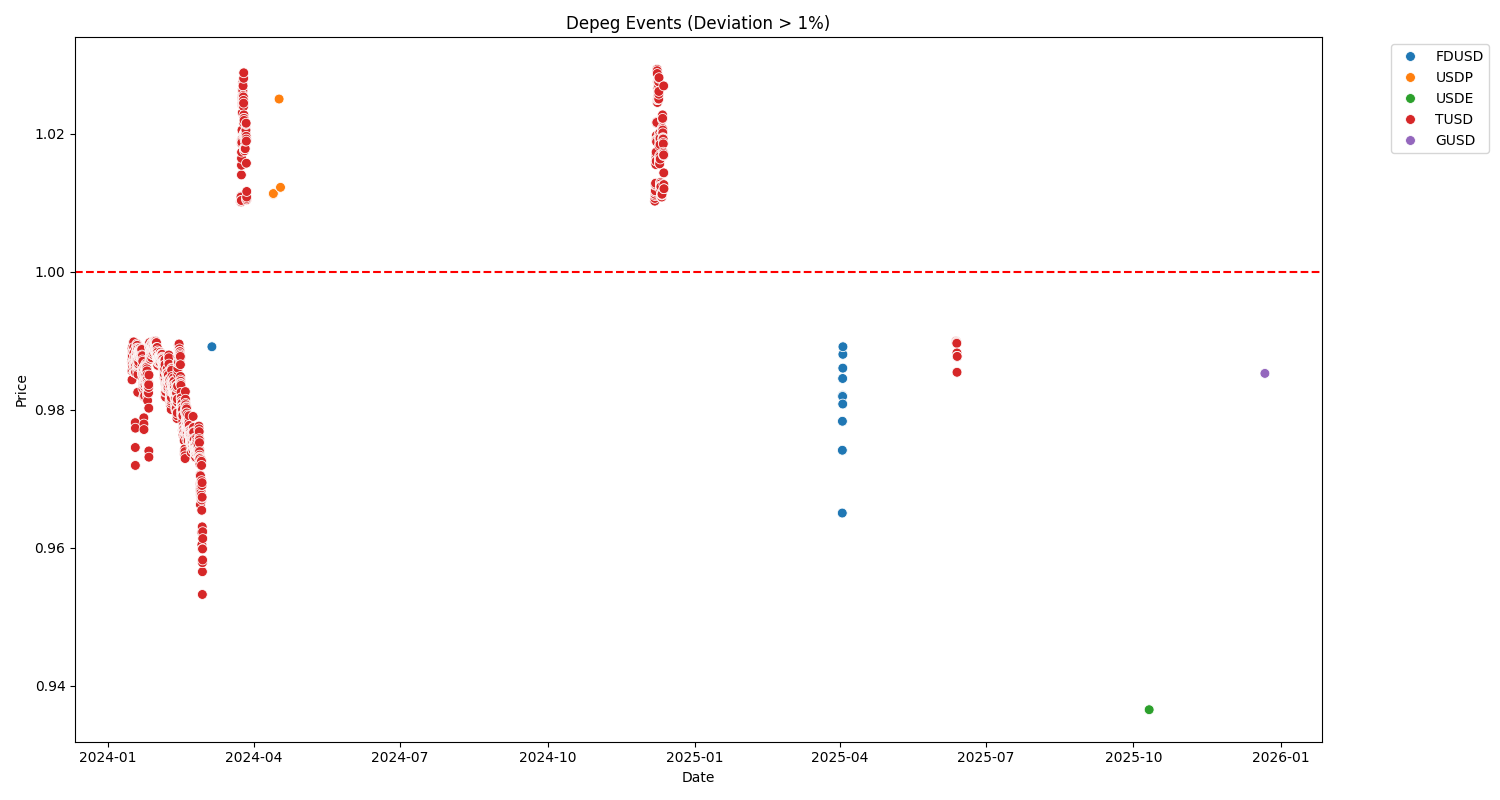
\includegraphics[width=\textwidth]{reports/figures/depeg_events.png}
    \caption{Historical depeg events (deviation $>$1\%).}
\end{figure}
\end{columns}
\end{frame}

% Slide 3: Data Overview
\begin{frame}{Data Collection \& Scope}
\begin{columns}[t]
\column{0.5\textwidth}
\textbf{Data Sources:}
\begin{itemize}
    \item \textbf{Coinbase:} USDT/USD, DAI/USD
    \item \textbf{Binance:} TUSD, FDUSD, USDP, USDE (vs USDT)
    \item \textbf{Context:} BTC/USD, ETH/USD for correlation
\end{itemize}

\vspace{0.2cm}
\textbf{Dataset Statistics:}
\begin{itemize}
    \item \textbf{Time Range:} $\sim$2 years hourly data
    \item \textbf{Records:} 89,003 observations
    \item \textbf{Train/Test:} 70,792 / 18,211
    \item \textbf{Depegs:} 1,271 events ($>$1\%)
\end{itemize}

\column{0.5\textwidth}
\textbf{Assets Processed:}
\begin{table}[h]
\footnotesize
\begin{tabular}{lll}
\toprule
\textbf{Coin} & \textbf{Exchange} & \textbf{Status} \\
\midrule
USDT, DAI & Coinbase & \textcolor{winnergreen}{\checkmark} \\
TUSD, FDUSD & Binance & \textcolor{winnergreen}{\checkmark} \\
USDP, USDE & Binance & \textcolor{winnergreen}{\checkmark} \\
\midrule
BUSD/FRAX/GUSD & -- & \textcolor{alertred}{Skipped} \\
\bottomrule
\end{tabular}
\end{table}
\small Skipped assets had $<$600 rows of data.
\end{columns}
\end{frame}

% Slide 4: Feature Engineering
\begin{frame}{Feature Engineering: 34 Predictive Features}
\begin{columns}[t]
\column{0.33\textwidth}
\textbf{Price Features:}
\begin{itemize}
    \item Deviation from \$1 (abs \& \%)
    \item 24h rolling volatility
    \item Price momentum (1h/6h/24h)
    \item Deviation velocity (rate of change)
\end{itemize}

\column{0.33\textwidth}
\textbf{Volume Features:}
\begin{itemize}
    \item 24h moving average
    \item 24h standard deviation
    \item Volume velocity
    \item Volume z-score
\end{itemize}

\column{0.33\textwidth}
\textbf{Lag \& Context Features:}
\begin{itemize}
    \item Multi-hour lags (1, 2, 3, 6, 12, 24h)
    \item BTC/ETH prices \& returns
    \item 24h rolling correlations with BTC/ETH
    \item Deviation z-score
\end{itemize}
\end{columns}

\vspace{0.5cm}
\begin{block}{Prediction Targets}
\begin{itemize}
    \item \textbf{Classification:} Binary risk label -- ``Low'' (depeg risk $>$1\%) vs ``Not-Low''
    \item \textbf{Regression:} Continuous deviation percentage 1 hour ahead
\end{itemize}
\end{block}
\end{frame}

% Slide 5: Methodology
\begin{frame}{Methodology: Four ML Approaches}
\begin{columns}[t]
\column{0.5\textwidth}
\textbf{1. Unsupervised Learning:}
\begin{itemize}
    \item \textbf{Clustering:} Identify market regimes
    \begin{itemize}
        \item K-Means (3 clusters)
        \item DBSCAN (density-based)
    \end{itemize}
    \item \textbf{Anomaly Detection:} Flag potential depegs
    \begin{itemize}
        \item Isolation Forest
        \item Local Outlier Factor (LOF)
    \end{itemize}
\end{itemize}

\column{0.5\textwidth}
\textbf{2. Supervised Learning:}
\begin{itemize}
    \item \textbf{Classification:} Predict binary risk
    \begin{itemize}
        \item Random Forest (500 trees)
        \item Gradient Boosting (300 estimators)
    \end{itemize}
    \item \textbf{Regression:} Predict deviation magnitude
    \begin{itemize}
        \item Ridge Regression (weighted)
        \item Neural Network (MLP: 128-64)
    \end{itemize}
\end{itemize}
\end{columns}

\vspace{0.3cm}
\begin{block}{Handling Class Imbalance}
Only 1.5\% of samples are ``Low'' (depeg) class. We applied: (1) 10$\times$ oversampling of Low class, (2) class weights (1:20), (3) aggressive probability threshold (0.005).
\end{block}
\end{frame}

% Slide 6: EDA - Price History
\begin{frame}{Exploratory Analysis: Price Stability Varies by Stablecoin}
\begin{columns}
\column{0.55\textwidth}
\begin{figure}
    \centering
    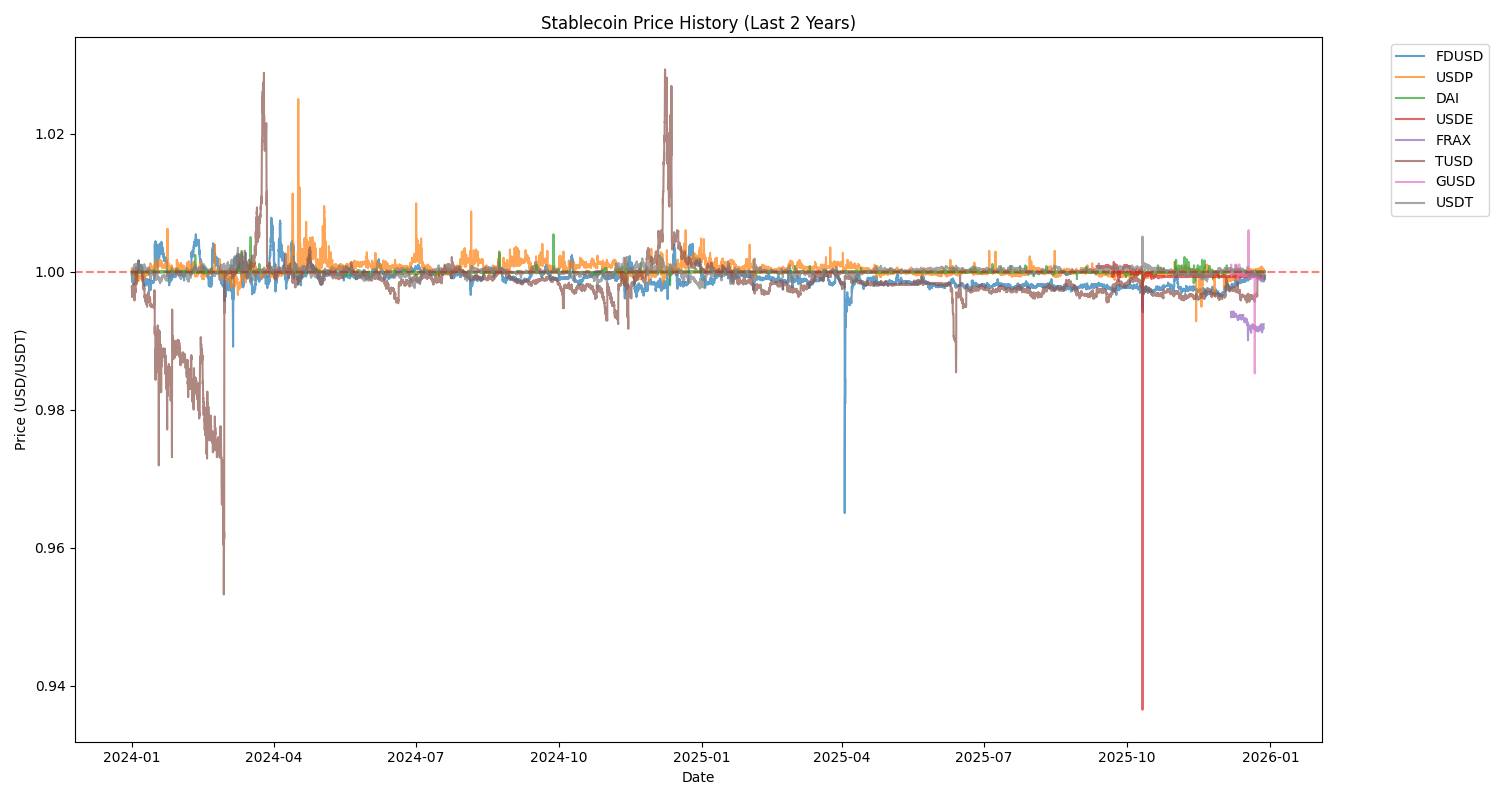
\includegraphics[width=\textwidth]{reports/figures/price_history.png}
    \caption{2-year price history across all stablecoins.}
\end{figure}

\column{0.45\textwidth}
\textbf{Key Observations:}
\begin{itemize}
    \item \textbf{USDT \& DAI:} Extremely stable, rarely deviate $>$0.1\%
    \item \textbf{TUSD:} Most volatile -- major depeg events visible
    \item \textbf{FDUSD/USDP/USDE:} Moderate fluctuations
\end{itemize}

\vspace{0.3cm}
\textbf{Implication:}
\begin{itemize}
    \item Models must handle both stable and volatile regimes
    \item Per-symbol evaluation critical for fair assessment
\end{itemize}
\end{columns}
\end{frame}

% Slide 7: EDA - Correlations
\begin{frame}{Exploratory Analysis: Cross-Asset Correlations}
\begin{columns}
\column{0.45\textwidth}
\begin{figure}
    \centering
    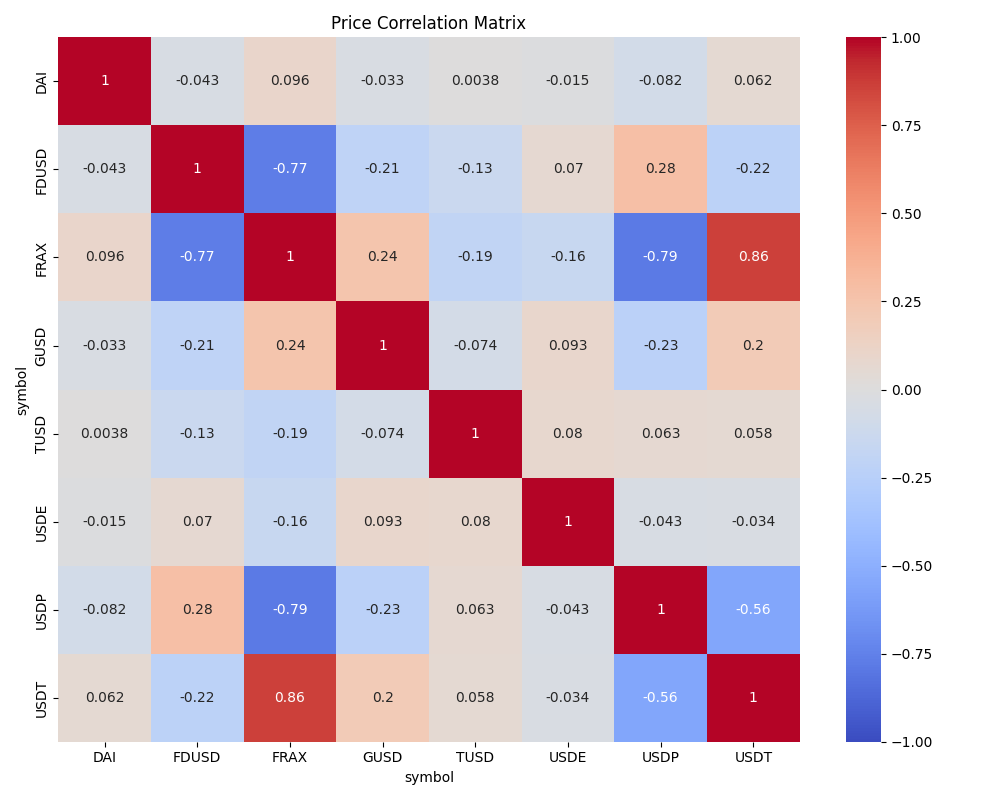
\includegraphics[width=\textwidth]{reports/figures/correlation_heatmap.png}
    \caption{Price correlation matrix.}
\end{figure}

\column{0.55\textwidth}
\textbf{Correlation Insights:}
\begin{itemize}
    \item Most stablecoins show \textbf{low correlation} with each other (independent behavior)
    \item \textbf{BTC \& ETH} are highly correlated (0.9+) as expected
    \item Stablecoin-crypto correlations are weak
    \begin{itemize}
        \item Suggests depegs are \textit{not} purely driven by market crashes
        \item Idiosyncratic factors (issuer risk, liquidity) matter
    \end{itemize}
\end{itemize}

\vspace{0.2cm}
\textbf{Feature Engineering Value:}\\
Including BTC/ETH context helps capture market-wide stress events that may precede depegs.
\end{columns}
\end{frame}

% Slide 8: Clustering Results
\begin{frame}{Clustering: Identifying Market Regimes}
\begin{columns}
\column{0.55\textwidth}
\begin{figure}
    \centering
    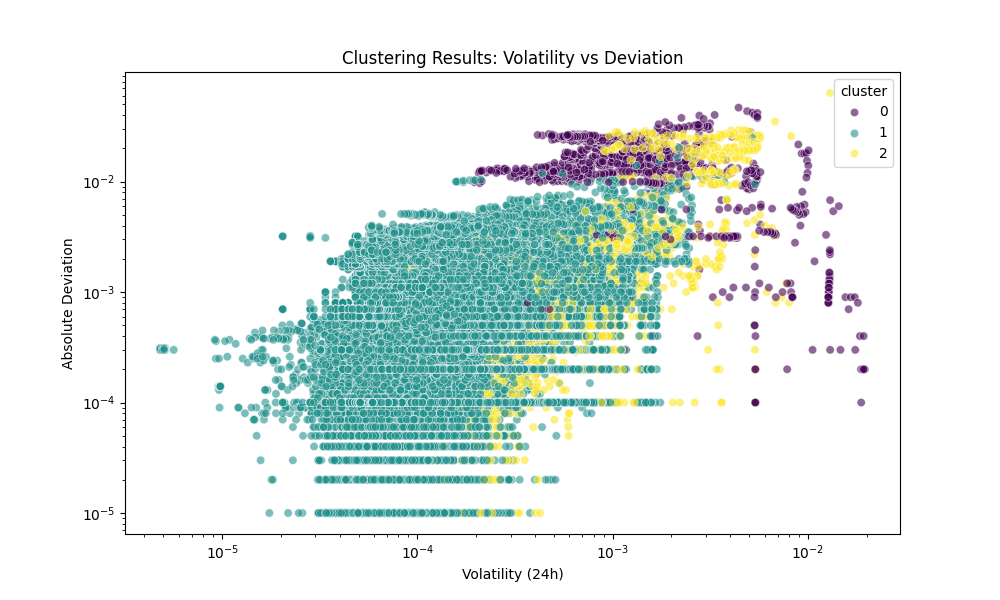
\includegraphics[width=\textwidth]{reports/figures/clustering_clusters.png}
    \caption{K-Means clusters: Volatility vs Deviation.}
\end{figure}

\column{0.45\textwidth}
\textbf{Model Comparison:}
\begin{table}[h]
\small
\begin{tabular}{lcc}
\toprule
\textbf{Metric} & \textbf{K-Means} & \textbf{DBSCAN} \\
\midrule
Clusters & 3 & 378 \\
Silhouette & \textbf{0.490} & 0.234 \\
Noise Points & 0 & 84,933 \\
\bottomrule
\end{tabular}
\end{table}

\textbf{3 Regimes Identified:}
\begin{itemize}
    \item \textbf{Stable:} Low volatility, minimal deviation
    \item \textbf{Moderate:} Elevated volatility
    \item \textbf{Stressed:} High volatility, large deviations
\end{itemize}

\textcolor{winnergreen}{\textbf{Winner: K-Means}} -- 2$\times$ better silhouette.
\end{columns}
\end{frame}

% Slide 9: Classification Results
\begin{frame}{Classification: Predicting Depeg Risk (1h Ahead)}
\begin{columns}
\column{0.4\textwidth}
\begin{figure}
    \centering
    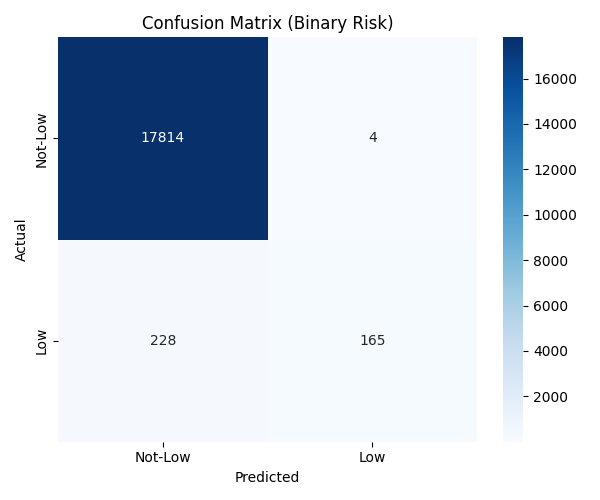
\includegraphics[width=\textwidth]{reports/figures/classification_confusion_matrix.png}
    \caption{Confusion matrix (Random Forest).}
\end{figure}

\column{0.6\textwidth}
\textbf{Model Comparison (Test Set: 18,211 samples):}
\begin{table}[h]
\small
\begin{tabular}{lcc}
\toprule
\textbf{Metric} & \textbf{Random Forest} & \textbf{Gradient Boosting} \\
\midrule
Accuracy & \textbf{98.73\%} & 98.61\% \\
F1 (weighted) & \textbf{0.985} & 0.983 \\
Low Precision & 98\% & \textbf{99\%} \\
Low Recall & \textbf{42\%} & 36\% \\
Low F1 & \textbf{0.59} & 0.53 \\
\bottomrule
\end{tabular}
\end{table}

\vspace{0.2cm}
\textbf{Per-Symbol Accuracy:}\\
\footnotesize DAI: 100\% | USDT: 100\% | FDUSD: 99.9\% | USDP: 99.9\% | USDE: 99.8\% | TUSD: 94.2\%

\vspace{0.2cm}
\normalsize\textcolor{winnergreen}{\textbf{Winner: Random Forest}} -- 17\% better recall on critical ``Low'' class (165 vs 142 true positives captured).
\end{columns}
\end{frame}

% Slide 10: Anomaly Detection Results
\begin{frame}{Anomaly Detection: Flagging Depeg Events}
\begin{columns}
\column{0.5\textwidth}
\begin{figure}
    \centering
    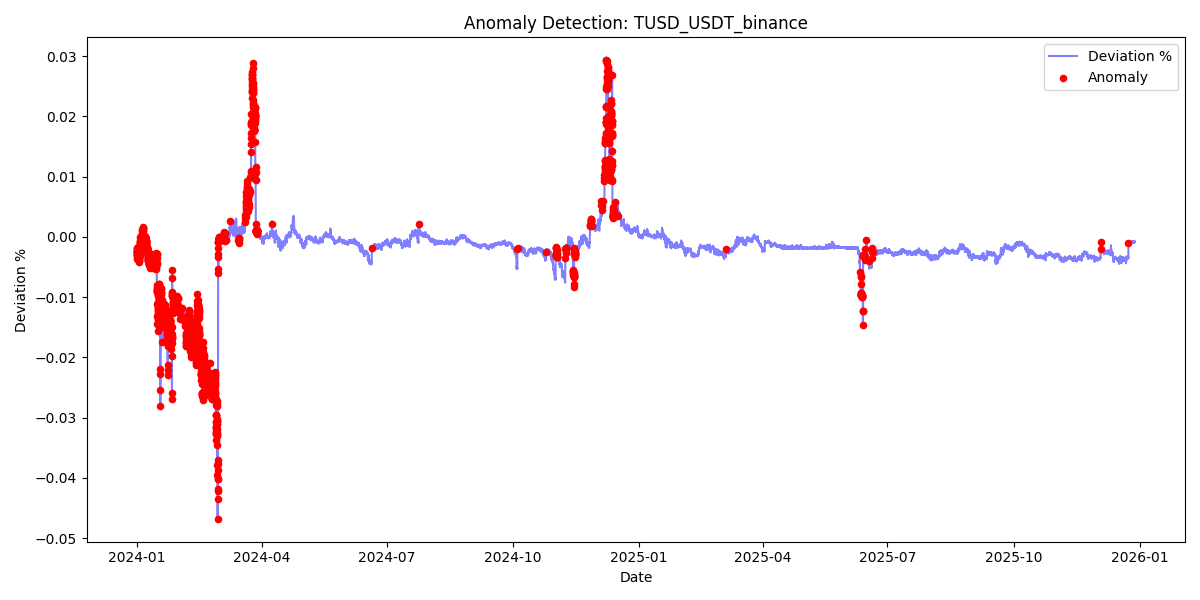
\includegraphics[width=\textwidth]{reports/figures/anomaly_detection_TUSD_USDT_binance.png}
    \caption{Isolation Forest anomalies on TUSD (most volatile).}
\end{figure}

\column{0.5\textwidth}
\textbf{Ground Truth:} 1,271 depeg events ($>$1\% deviation)

\vspace{0.3cm}
\textbf{Model Comparison:}
\begin{table}[h]
\small
\begin{tabular}{lcc}
\toprule
\textbf{Metric} & \textbf{Isolation Forest} & \textbf{LOF} \\
\midrule
Detected & 2,227 & 2,977 \\
Precision & \textbf{0.474} & 0.118 \\
Recall & \textbf{0.831} & 0.277 \\
F1 Score & \textbf{0.604} & 0.166 \\
\bottomrule
\end{tabular}
\end{table}

\vspace{0.2cm}
\textcolor{winnergreen}{\textbf{Winner: Isolation Forest}}
\begin{itemize}
    \item Captures \textbf{83\%} of true depegs
    \item 3.6$\times$ better F1 than LOF
    \item Per-symbol contamination tuning improved results
\end{itemize}
\end{columns}
\end{frame}

% Slide 11: Regression Results
\begin{frame}{Regression: Forecasting Deviation Magnitude (+1h)}
\begin{columns}
\column{0.5\textwidth}
\begin{figure}
    \centering
    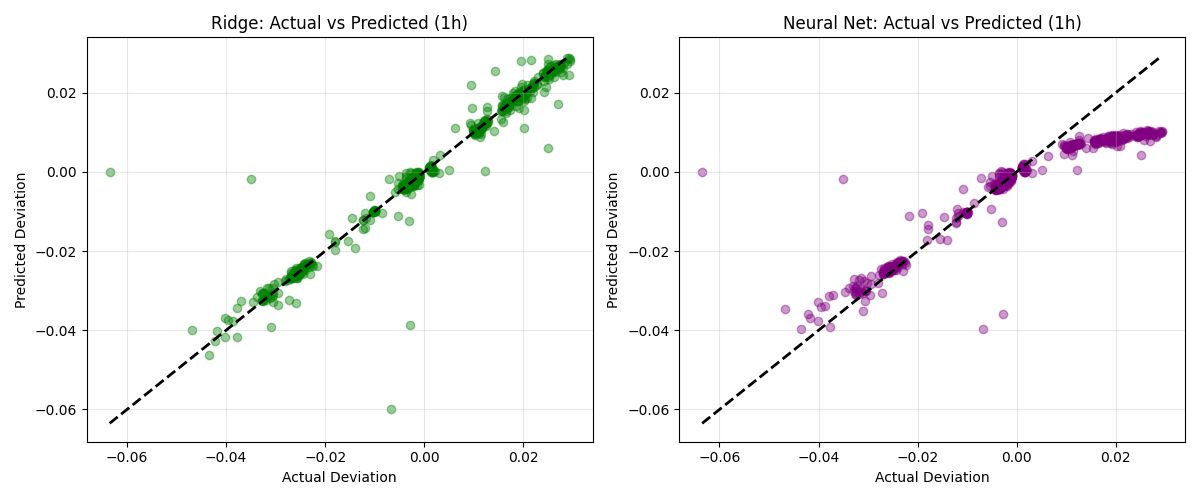
\includegraphics[width=\textwidth]{reports/figures/regression_vs_nn_scatter.png}
    \caption{Predicted vs actual deviation (Ridge \& NN).}
\end{figure}

\column{0.5\textwidth}
\textbf{Global Performance:}
\begin{table}[h]
\small
\begin{tabular}{lcc}
\toprule
\textbf{Metric} & \textbf{Ridge} & \textbf{Neural Net} \\
\midrule
RMSE & \textbf{0.00081} & 0.00149 \\
R\(^2\) & \textbf{0.951} & 0.834 \\
\bottomrule
\end{tabular}
\end{table}

\vspace{0.2cm}
\textbf{Per-Symbol R\(^2\):}
\begin{table}[h]
\footnotesize
\begin{tabular}{lc|lc}
\toprule
Symbol & R\(^2\) & Symbol & R\(^2\) \\
\midrule
TUSD & \textbf{0.987} & FDUSD & 0.738 \\
USDT & 0.911 & USDP & 0.557 \\
DAI & -0.024 & USDE & -0.725 \\
\bottomrule
\end{tabular}
\end{table}

\textcolor{winnergreen}{\textbf{Winner: Ridge Regression}} -- 1.8$\times$ lower RMSE, simpler model generalizes better.
\end{columns}
\end{frame}

% Slide 12: Key Findings
\begin{frame}{Key Findings \& Conclusions}
\begin{columns}[t]
\column{0.5\textwidth}
\textbf{Model Performance:}
\begin{itemize}
    \item \textbf{Clustering:} K-Means finds 3 market regimes
    \item \textbf{Classification:} RF achieves 98.7\% accuracy, 42\% recall on depegs
    \item \textbf{Anomaly:} IsoForest captures 83\% of depegs (F1=0.60)
    \item \textbf{Regression:} Ridge achieves R\(^2\)=0.95
\end{itemize}

\column{0.5\textwidth}
\textbf{Insights:}
\begin{itemize}
    \item TUSD shows frequent depegs; DAI/USDT are stable
    \item Volatile coins easier to forecast (TUSD: R\(^2\)=0.99)
    \item Class imbalance requires aggressive handling
    \item Simpler models win: Ridge $>$ NN, K-Means $>$ DBSCAN
\end{itemize}
\end{columns}

\vspace{0.2cm}
\begin{block}{Practical Application}
IsoForest + Ridge can form a real-time alert system: flag anomalies (83\% recall), then quantify expected deviation (R\(^2\)=0.95).
\end{block}
\end{frame}

% Slide 13: Technical Summary
\begin{frame}{Technical Summary}
\begin{columns}[t]
\column{0.5\textwidth}
\textbf{Implementation:}
\begin{itemize}
    \item \textbf{Data:} \texttt{ccxt} for exchange APIs
    \item \textbf{ML:} scikit-learn (K-Means, RF, Ridge, IsoForest, MLP)
    \item \textbf{Viz:} matplotlib, seaborn, plotly
\end{itemize}

\vspace{0.2cm}
\textbf{Codebase:}
\begin{itemize}
    \item \texttt{src/data\_collector.py}
    \item \texttt{src/preprocessor.py}
    \item \texttt{src/modeling.py}
    \item \texttt{src/visualization.py}
\end{itemize}

\column{0.5\textwidth}
\textbf{Final Metrics:}
\begin{table}[h]
\small
\begin{tabular}{ll}
\toprule
\textbf{Task} & \textbf{Best Result} \\
\midrule
Clustering & Silhouette 0.490 \\
Classification & Acc 98.7\%, F1 0.59 \\
Anomaly & F1 0.60, Recall 83\% \\
Regression & R\(^2\) 0.95, RMSE 0.0008 \\
\bottomrule
\end{tabular}
\end{table}

\vspace{0.2cm}
\textbf{Best Models:} K-Means, Random Forest, Isolation Forest, Ridge Regression
\end{columns}
\end{frame}

% Slide 14: Q&A
\begin{frame}[plain]
\begin{center}
\Huge \textbf{Thank You!}

\vspace{0.8cm}

\normalsize

\vspace{0.5cm}

\textbf{Contact:}\\
\texttt{eymen.celikturk@std.bogazici.edu.tr}\\
\texttt{halil.celik@std.bogazici.edu.tr}

\end{center}
\end{frame}

\end{document}
